\chapter{Présentation de la maquette}

\section{Présentation de la maquette}

\section{Fonctionnement de la maquette}

\section{Présentation de l'électronique}

\section{Première mise en service}
Une première mise en service a été réalisée afin d'observer l'état de l'électronique. Pour ce faire, la mise en place ainsi que le protocole détaillé dans les sections \ref{sec:MiseEnPlace} et \ref{sec:Protocole} ont été suivis. Une vérification plus approfondie de l'électronique est par ailleurs réalisée dans le chapitre 4.

\subsection{Vérification de la charge du condensateur}
Le condensateur a été vérifié afin de comparer le résultat obtenu à celui de Thomas Freyche, illustré dans la figure \ref{fig:ResFreycheCapa} :

\begin{figure}[H]
    \centering
    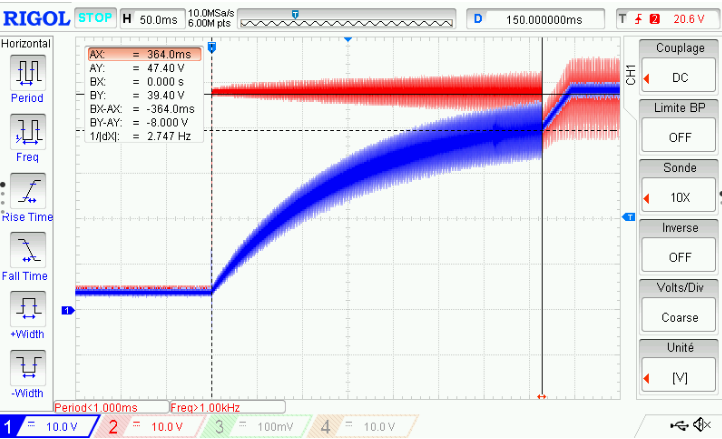
\includegraphics[width=0.75\linewidth]{Image/Chap.3/Result_Freyche_Capa.png}
    \caption{Résultat de la mesure du condensateur du rapport de Thomas Freyche}
    \label{fig:ResFreycheCapa}
\end{figure}

Lors de la mesure effectuée pour ce travail, un résultat identique a été obtenu, comme le montre la figure \ref{fig:ResCanCapa} :

\begin{figure}[H]
    \centering
    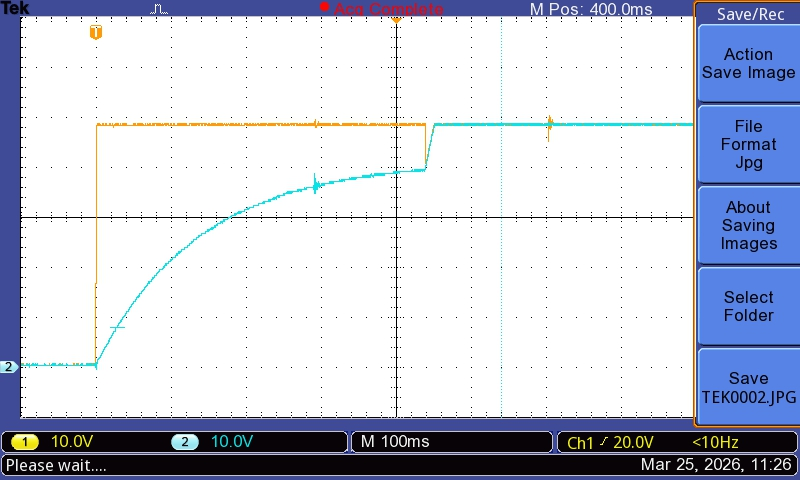
\includegraphics[width=0.75\linewidth]{Image/Chap.3/MesureCondoCan.JPG}
    \caption{Résultat de la mesure du condensateur personnel}
    \label{fig:ResCanCapa}
\end{figure}

\subsection{Constats et diagnostic de fonctionnement}
Dès la mise sous tension, le fonctionnement de l'électronique est partiellement validé par le soulèvement effectif des inducteurs. Cependant, la régulation ne semble pas opérationnelle. Ce constat pointe vers un problème potentiel situé soit au niveau logiciel (software), soit au niveau matériel (hardware).

Cette étape constitue tout de même un point de départ encourageant, car elle permet de cibler la partie causant les dysfonctionnements. Les différentes hypothèses de résolution seront détaillées dans la sous-section \ref{sec:Hypothese}.

\section{Mesure de la carte principale}